\subsection{Building Blocks}\label{subsec:Building_Blocks}
Although the virtual machine concept is useful, it is difficult to implement.
Much work is required to provide an exact duplicate of the underlying machine.
This is especially a challenge on dual-mode systems, where the underlying machine has only user mode and kernel mode.

\begin{remark*}
  Note that these building blocks are not required by \nameref{def:Type0_Hypervisor}s.
\end{remark*}

The ability to virtualize heavily depends on the hardware features provided by the CPU.\@
If the features are sufficient, then it is possible to write a \nameref{def:VMM} that provides a guest environment.
Otherwise, \nameref{def:Virtualization} is impossible.

If it is possible to virtualize a system, the \nameref{def:VMM}s use several techniques to implement it, including \nameref{subsubsec:Trap_and_Emulate} and \nameref{subsubsec:Binary_Translation}.

One important concept found in most virtualization options is the implementation of a \nameref{def:Virtual_CPU}.

\begin{definition}[Virtual CPU]\label{def:Virtual_CPU}\label{def:VCPU}
  The \emph{Virtual CPU} (\emph{VCPU}) does not execute code.
  Rather, it represents the state of the guest's CPU as the guest machine believes it to be.
  For each guest, the VMM maintains a VCPU representing that guest's current CPU state, much like a \nameref{def:Process_Control_Block}.
  When the guest is \nameref{def:Context_Switch}ed onto a physical CPU by the \nameref{def:VMM}, information from the VCPU is used to load the right context, much as a general-purpose \nameref{def:Operating_System} would use the PCB.\@
\end{definition}

\subsubsection{Trap-and-Emulate}\label{subsubsec:Trap_and_Emulate}
On a typical dual-mode system, the virtual machine guest can execute only in user mode (unless extra hardware support is provided).
The kernel, of course, runs in kernel mode, and it is not safe to allow user-level code to run in kernel mode.
Just as the physical machine has two modes, however, so must the virtual machine.
Consequently, we must have a virtual user mode and a virtual kernel mode, both of which run in physical user mode.
Actions that cause a transfer from user mode to kernel mode on a real machine (such as a \nameref{def:System_Call}, an \nameref{def:Interrupt}, or an attempt to execute a privileged instruction) must also cause a transfer from virtual user-mode to virtual kernel-mode in the \nameref{def:Virtual_Machine}.

When the kernel in the guest attempts to execute a privileged instruction, that is an error (because the system is in both physical user-mode and virtual user-mode) and causes a trap to the \nameref{def:VMM} in the real machine.
The VMM gains control and executes (or ``emulates'') the action that was attempted by the guest kernel on the part of the guest.
It then returns control to the \nameref{def:Virtual_Machine}.

With privileged instructions, time becomes an issue.
All nonprivileged instructions run natively on the \nameref{def:Hardware}, providing the same performance for guests as native applications.
Privileged instructions create extra overhead, causing the guest to run more slowly than it would natively.
In addition, the CPU is being multiprogrammed among many \nameref{def:Virtual_Machine}s, which can further slow down the virtual machines in unpredictable ways.

Only the privileged instructions (needed mainly for I/O) must be emulated and hence only these instructions execute more slowly.
In general, with the evolution of hardware, the performance of trap-and-emulate functionality has been improved, and cases in which it is needed have been reduced.
For example, many CPUs now have extra modes added to their standard dual-mode operation.

\subsubsection{Binary Translation}\label{subsubsec:Binary_Translation}
Some CPUs do not have a clean separation of privileged and nonprivileged instructions.
This includes the Intel x86 CPU line, which started in 1978.
The chip has maintained backward compatibility throughout its lifetime, preventing changes that would have made virtualization easier through many generations.

For example, \texttt{popf} instruction loads the flag register from the contents of the stack.
If the CPU is in privileged mode, \textbf{all} of the flags are replaced from the stack.
If the CPU is in user mode, then only some flags are replaced, and others are ignored.
Because no trap is generated if \texttt{popf} is executed in user mode, the \nameref{subsubsec:Trap_and_Emulate} procedure is rendered useless.
Other x86 instructions cause similar problems.
These instructions will be refered to as \textbf{special instructions}.
As recently as 1998, it seemed that using the trap-and-emulate method to implement \nameref{def:Virtualization} on the x86 was considered impossible because of these special instructions.

Binary translation is fairly simple in concept but complex in implementation.
The basic steps are as follows:
\begin{enumerate}[noitemsep]
\item If the guest VCPU is in user mode, the guest can run its instructions natively on a physical CPU.\@
\item If the guest VCPU is in kernel mode, then the guest believes that it is running in kernel mode.
  The \nameref{def:VMM} examines every instruction the guest executes in virtual kernel mode by reading the next few instructions that the guest is going to execute, based on the guest's program counter.
  Instructions other than special instructions are run natively.
  Special instructions are translated into a new set of instructions that perform the equivalent task—for example changing the flags in the VCPU.\@
\end{enumerate}

This basic method of binary translation just described would execute correctly but perform poorly.
Fortunately, the vast majority of instructions would execute natively.
Caching of previously translated instructions can provide further increases to performance, particularly if the cache is large enough.

\subsubsection{Hardware Assistance}\label{subsubsec:VM_Hardware_Assistance}
Without some level of hardware support, virtualization would be impossible.
The more hardware support available within a system, the more feature-rich and stable the virtual machines can be and the better they can perform.

For example, AMD \nameref{def:Virtualization} technology (AMD-V) defines two additional modes of operation: host and guest.
This makes these CPUs multimode processors, rather than dual-mode.
The \nameref{def:VMM} can enable host mode, define the characteristics of each guest \nameref{def:Virtual_Machine}, and then switch the system to guest mode, passing control of the system to a guest operating system that is running in the virtual machine.
In guest mode, the virtualized operating system thinks it is running on native hardware and sees whatever devices are included in the host's definition of the guest.
If the guest tries to access a virtualized resource, then control is passed to the VMM to manage that interaction.

These multimode processors, developed for \nameref{def:Virtualization} provide guest \nameref{def:VCPU} state data structures to load and save guest CPU state automatically during guest context switches.
In addition, virtual machine control structures (VMCSs) are provided to manage guest and host state, as well as the various guest execution controls, exit controls, and information about why guests exit back to the host.

AMD and Intel have also addressed memory management in the virtual environment.
With these memory management enhancements, VMMs no longer need to implement software Nested Page Tables (NPTs).
These CPUs implement nested page tables in hardware to allow the VMM to fully control paging while the CPUs accelerate the translation from virtual to physical addresses.
The NPTs add a new layer, one representing the guest's view of logical-to-physical address translation.
The CPU page-table walking function includes this new layer as necessary, walking through the guest table to the VMM table to find the physical address desired.
This process is illustrated in \Cref{fig:Nested_Page_Tables}.

\begin{figure}[h!tbp]
  \centering
  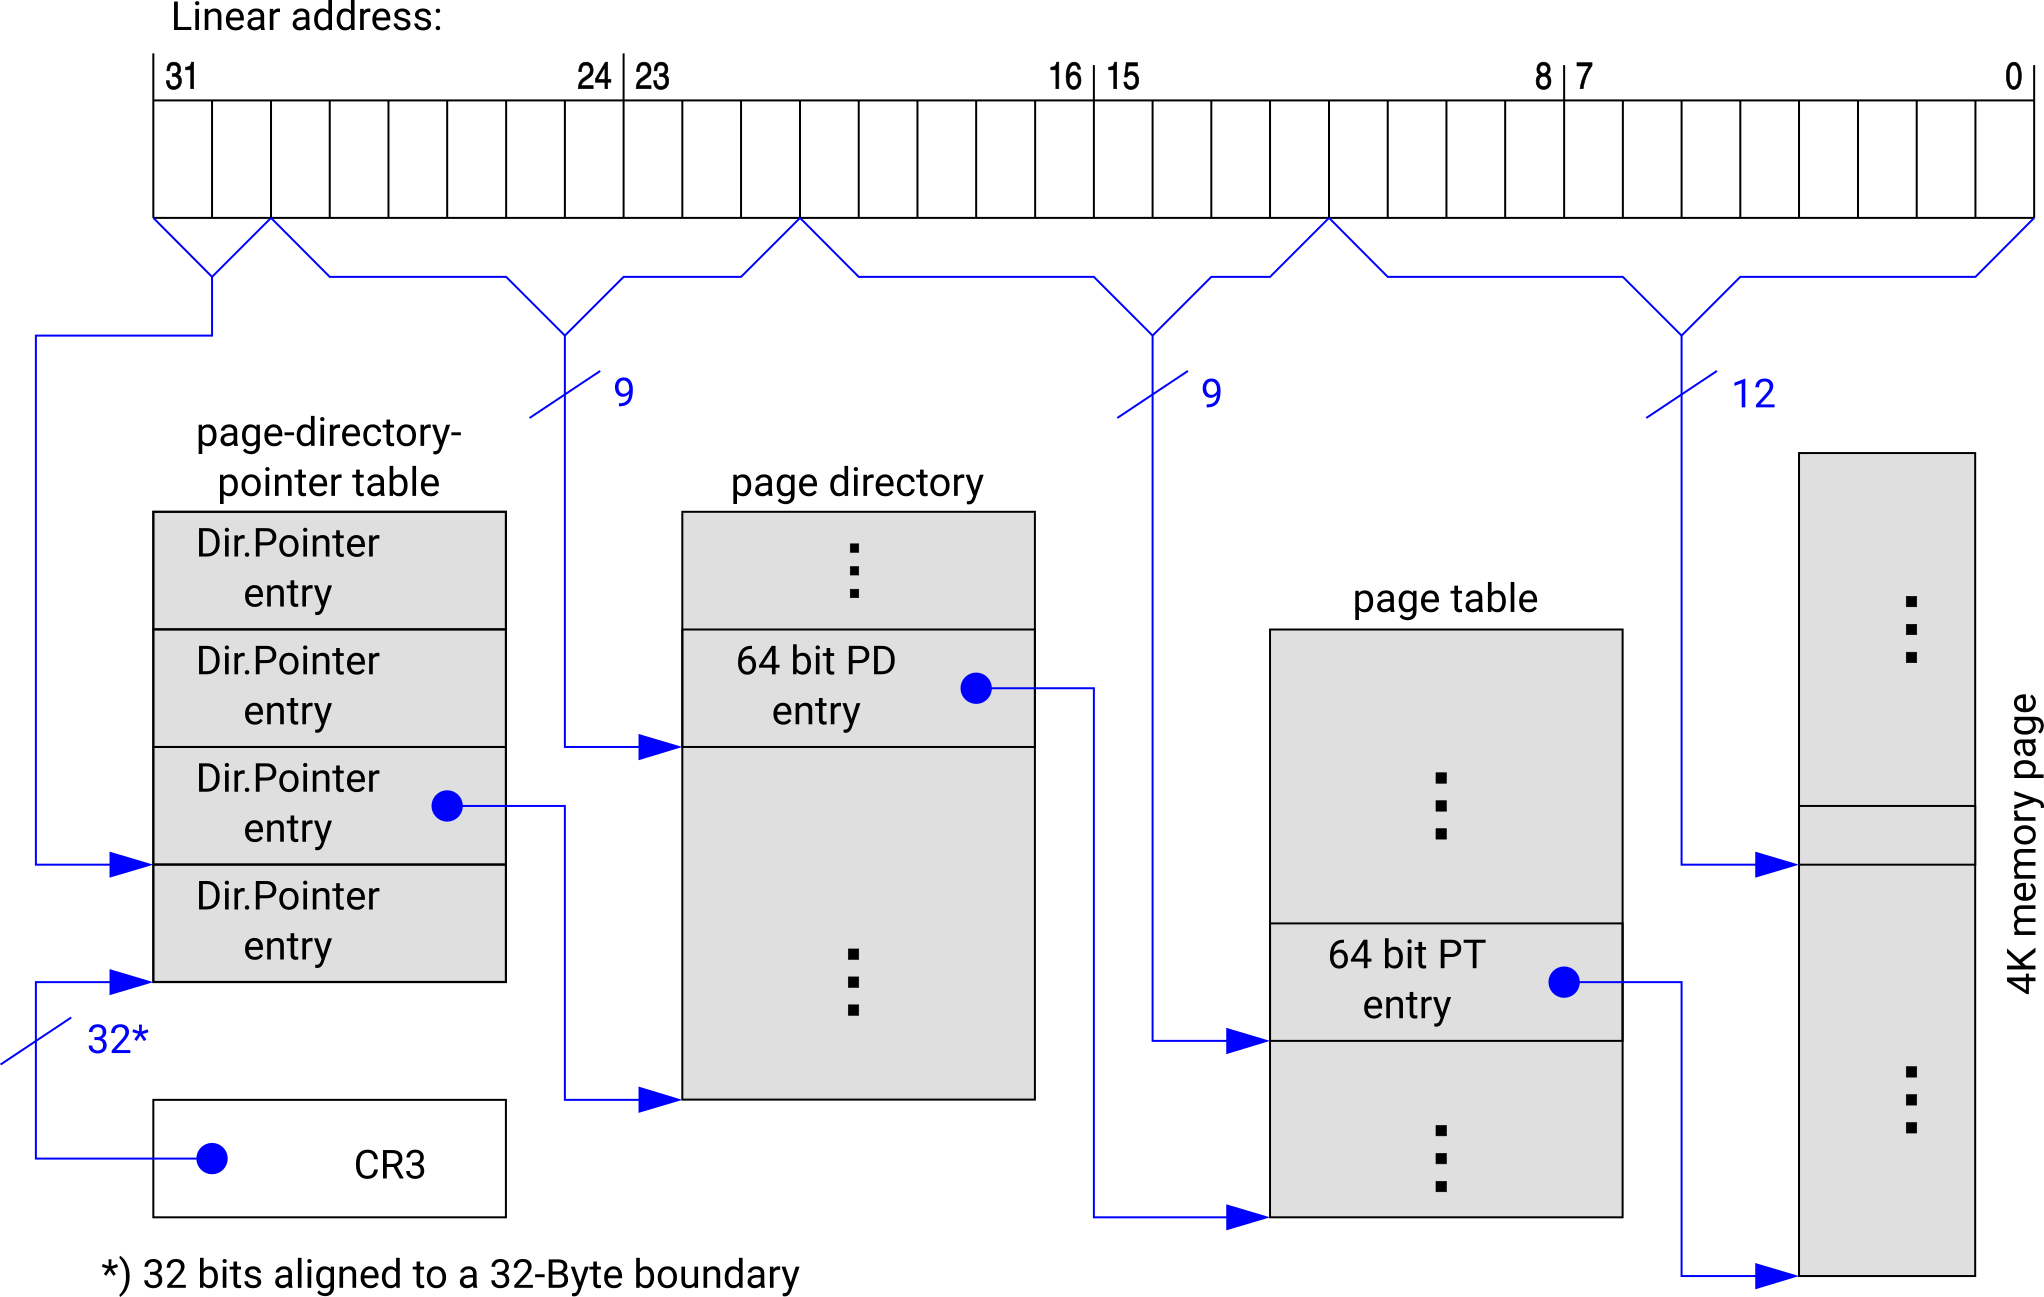
\includegraphics[scale=1.00]{./Drawings/EDAF35-Operating_Systems/Nested_Page_Tables-Virtualization.png}
  \caption{Nested Page Tables, for Virtualization}
  \label{fig:Nested_Page_Tables}
\end{figure}



%%% Local Variables:
%%% mode: latex
%%% TeX-master: "../../EDAF35-Operating_Systems-Reference_Sheet"
%%% End:
